The major usage of \gls{JIT} compilation by \gls{PyExaFMM} is for the construction
of the Octree, including the calculation of the interaction lists for target
boxes, and to accelerate functions for its traversal. Computing the interaction list
involves looping over all target boxes of an octree, at all levels, therefore
is a good candidate for application of \gls{JIT} compilation. For benchmarking
we construct a three level octree, with 1000 randomly distributed particles which are
taken to be sources as well as targets. We report that without \gls{JIT} compilation
it takes $380 \pm 20$ ms, with errors taken as the standard deviation
and reported to 1 s.f over 5 runs; in comparison
to $8.2 \pm 0.9$ ms for the same experiment run with \gls{JIT} compilation.
\gls{JIT} compilation is also used to cache tree traversal methods, for example
used to calculate the parent box of a given box, or the level of the octree that
it is at. We benchmark the efficacy of this cache by computing the level
of a box with a Morton key of $1 \times 10^8$, for which we report \gls{JIT} compilation
takes $1 \pm 1$ µs with errors taken as the standard deviation and reported
to 1 s.f over 5 runs, in comparison to the ordinary Numpy implementation which takes
$3 µs ± 1 µs$ for the same experiment. The large errors for the \gls{JIT} compiled
function is indicative of the impact of the cache, with the the initial
run taking 10 times longer than the fastest one, reported to 1 s.f.

To benchmark the efficacy of HDF5 in comparison to serialisation for saving
and loading data from disk we create a Numpy array composed of
20,000 columns and 10,000 rows of 64 bit floats. This array has a minimum size
of 1.5 GB (1 s.f.), excluding the metadata associated with the type, and is
saved and loaded 5 times from disk for statistics. Serialisation throughout
\gls{PyExaFMM} is computed using the core Python Pickle library. For saving,
serialisation takes $2.7 \pm 0.7$ s (1 s.f), and hdf5 takes $1.1 \pm 0.2$ s (1 s.f).
For loading from memory, as HDF5's mechanism of returning a database style interface
rather than loading everything to disk, leads to the appearance of rapid
load times, we also measure the time taken to load the entire file to disk from
HDF5. Loading the serialised file takes $3.2 \pm 0.4$ s (1 s.f), loading
the HDF5 file to disk takes $1.4 \pm 0.1$ s (1 s.f). Using HDF5 is almost
twice as fast as serialisation, the reasons for this are due to the underlying
techniques used by each method. Roughly speaking, HDF5 stores raw numeric data
alongside a header file describing its dimensions, as a contiguous byte stream
on disk which allows for optimised methods to quickly search and retrieve data
\cite{collette2013python}. Object serialisation is designed to work with arbitrary
Python objects, raw numeric data is not stored, rather it is first compressed
into an intermediate representation, that results in a byte stream which is then
stored on disk. This data is stored alongside the metadata for the object, such
as it's initialisation code, and even any dependent objects it may have. The
intermediate representation allows any objects to be serialised in the same
manner \cite{pickle}.

Due to the constraints of accessible computing power, we benchmark the effect of
multiprocessing on operator matrix precomputation calculations using, a 3 level
non-adaptive octree, containing 1000 randomly distributed
particles placed in a unit cube which are used as sources as well as targets,
using the Laplace kernel from our model problem (\ref{eq:electrostatic_paradigm}).
Furthermore, all sources are given a charge density of 1 Coulomb and the relevant surfaces
are calculated to order $p=2$, therefore each discretised with $8$ quadrature points
(\ref{eq:2_2_quadrature_points}), with the parameters for the relative sizes
of different surfaces are the same as those provided
in Chapter \ref{chpt:2_strategy_for_practical_implementation},
Section \ref{sec:2_3_operator_caching}.

We benchmark the efficacy of multiprocessing for accelerating the precomputation
of the \gls{M2M}, \gls{L2L} and \gls{M2L} operator matrices for the above octree
using different numbers of \gls{CPU} processor cores in figure (\ref{fig:3_1_multiproc}).
Operators are computed three times for a given number of processor cores
for statistics. The speedup offered by increasing the number of processor cores
is non-linear, this is indicative of a communication overhead, and the
fact that multiprocessing has been implemented to a very basic degree with
the required data being copied to each process, even if very large.

\begin{figure}[ht]
    \centering

  {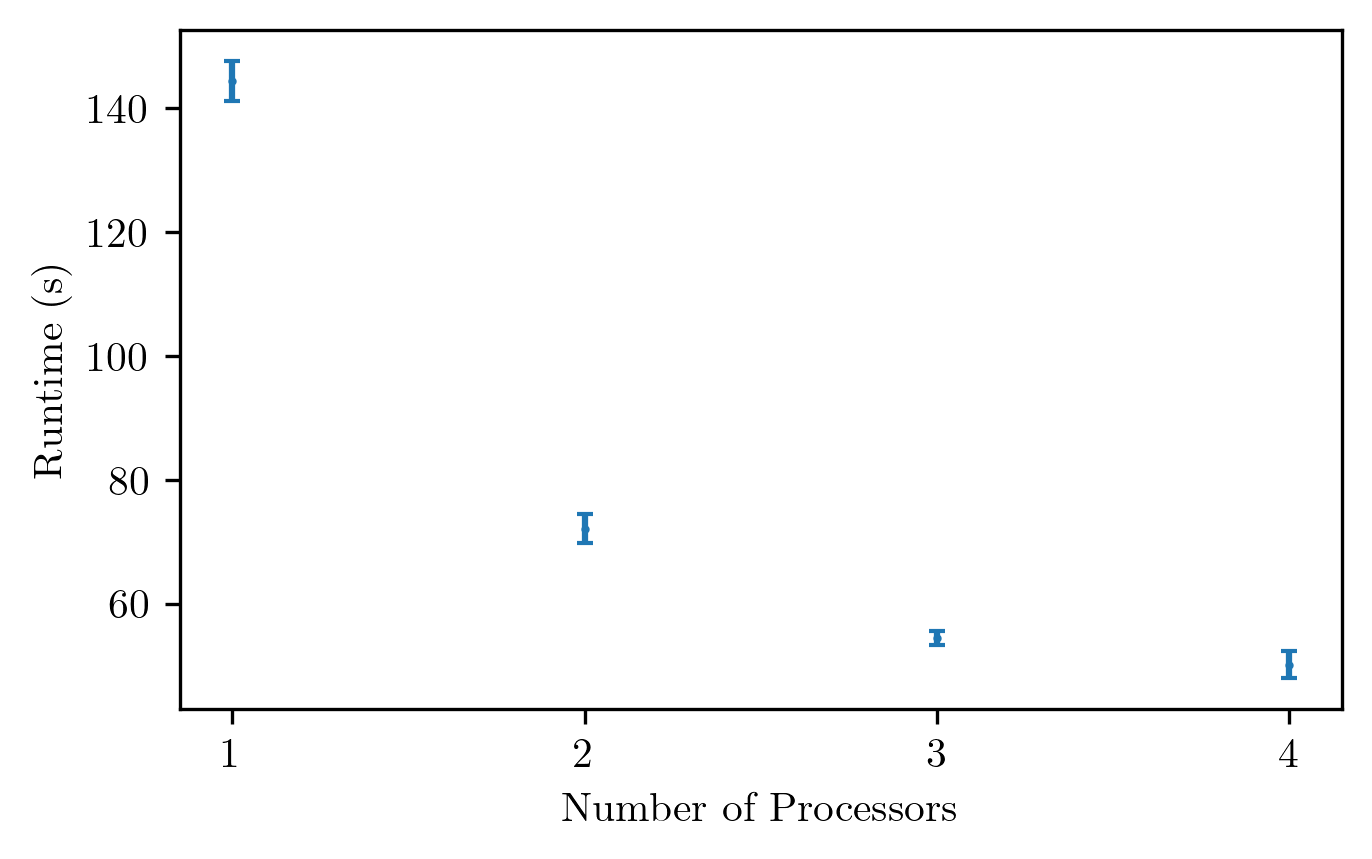
\includegraphics[width=0.9\textwidth]{chapter3/multiproc.png}}
  \vspace{0pt}
    \caption{Runtime versus number of processors used for operator precomputations
    for the model problem (\ref{eq:electrostatic_paradigm}). Error bars are
    plotted using standard deviation.
    }
    \label{fig:3_1_multiproc}
\end{figure}

We benchmark the algorithm run time in comparison to direct computation in figure
(\ref{fig:3_1_complexity}), with same parameters as the octree used for benchmarking
the operator precomputation, but with an increasing number of target and source
particles $N$ for our model problem (\ref{eq:electrostatic_paradigm}). The
calculations are run three times for each problem size for statistics.
Assuming a power relationship between run time $t$ and problem size $N$,

\begin{equation}
    t = N^x
\end{equation}

where $x$ is unknown, taking logarithms allows one to apply least squares fitting
to fit a linear relationship to,

\begin{equation}
    \log(t) = x \log(N)
\end{equation}

computing the value of $x$ from the gradient. Performing this calculation for the
results from the \gls{FMM} and direct approaches we report $x=1.14$ (2 d.p) for
the FMM, and $x=1.98$ (2 d.p) for the direct method. This implies an approximate
asymptotic complexity of $O(N)$, and $O(N^2)$ for the \gls{FMM} and direct methods
respectively in line with what is expected, with the limitation that this has
been tested on relatively small inputs of only $O(10^3)$ particles.

\begin{figure}[ht]
    \centering

  {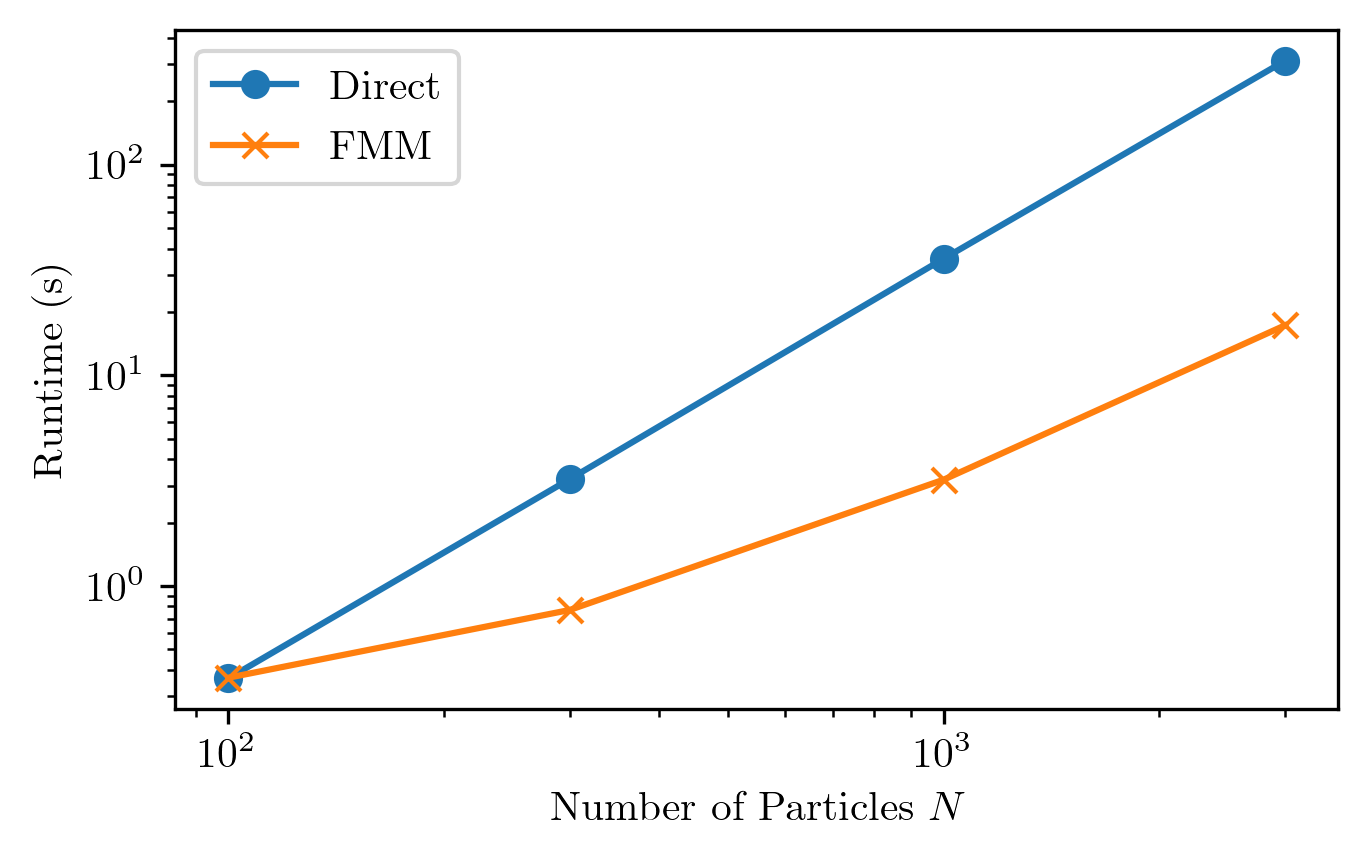
\includegraphics[width=0.9\textwidth]{chapter3/complexity.png}}
  \vspace{0pt}
    \caption{
        Runtime versus problem size to solve the model problem
        (\ref{eq:electrostatic_paradigm}) using direct calculations and
        \gls{PyExaFMM}.
    }
    \label{fig:3_1_complexity}
\end{figure}

In terms of a benchmark figure, we can report that with a simulation with
the above octree and $N=3000$ takes $17.1 \pm 0.2$ s, over the three runs with
error calculated from standard deviation and reported to 1 s.f. From correspondence
with the authors of ExaFMM-T, we can report their corresponding benchmark figure,
calculated on a 14 Core Intel i9-7940X \gls{CPU} with $N=10^6$ particles
randomly distributed in a unit cube, it takes 0.52 s to perform a $p=4$ degree
computation, including tree construction but excluding the
operator precomputations, in single precision. Time limitations for this project
makes it difficult to perform comparisons using equivalent hardware, however
disparities in hardware are unlikely to explain the magnitude of superiority
of ExaFMM-t's performance in comparison to \gls{PyExaFMM}.

ExaFMM-T implements a range of optimisations which represent future avenues
of software development for \gls{PyExaFMM}. Specifically, they distribute the
\gls{P2P} and \gls{M2L} operations on \gls{GPU}s, as discussed in Chapter
\ref{chpt:2_strategy_for_practical_implementation},
Section \ref{sec:2_3_operator_caching}, as well as using \gls{OpenMP} to share
precomputed surfaces across processes in the operator precomputations.
\gls{PyExaFMM} does not distribute any calculations on \gls{GPU}s, and
wastefully copies surface data to each process for the operator precomputations.
Furthermore, ExaFMM-t optimises the application of the kernel function,
firstly by the inverse operation in (\ref{eq:electrostatic_paradigm}) using a Newton
iteration to approximate $x = 0.5x(w-ax^2)$ to approximate $x \approx a ^{-1/2}$,
the computation for which highly-optimised implementations exist
\cite{Lomont:2003, sqrt}. Secondly \textbf{\gls{AVX}} vectorisation is used
to apply the kernel function. Roughly speaking, \gls{AVX} vectorisation allows
for parallel execution of \gls{SIMD} type instructions in a \gls{CPU}. With similar
optimisations, PVFMM is able to report a 3.8 multiplicative speed up, in
comparison to naive applications of the Laplace kernel \cite{Malhotra:2015:CCP}.
